\documentclass[11pt,a4paper]{article}  % Déclare la classe du document.

\newcommand{\chaptermark}[2]{\og #2 \fg{} (#1)} % ligne uniquement pour éviter une erreur en cas d'article
\usepackage[table,dvipsnames,svgnames]{xcolor}
\usepackage{listingsutf8}
%\usepackage[utf8]{inputenc}% gestion des accents (source)
\usepackage[T1]{fontenc}% gestion des accents (PDF)
\usepackage{fontspec}
\usepackage[french]{babel}% gestion du français
\usepackage{textcomp}% caractères additionnels
\usepackage{mathtools,amssymb,amsthm}% packages de l'AMS + mathtools
\usepackage{amsmath}
\usepackage{yhmath}
\usepackage{mathpazo}
\usepackage[scaled=0.95]{helvet}
\usepackage{courier}
%\usepackage{fourier}
%\usepackage[scaled=0.95]{helvet}
%\usepackage{courier}
\usepackage{bm}
\usepackage{gensymb}
\usepackage{graphicx}

\usepackage{enumitem}
\usepackage{pifont}

\usepackage{pstricks}
\usepackage{pstricks-add}
\usepackage{pst-eucl}
\usepackage{pgfplots}
\let\clipbox\relax
%\usepackage{pst-plot,pst-text,pst-tree,pstricks-add}
%\usepackage{pst-node} % required package
\usepackage{pst-all}
\usepackage[most,skins,breakable]{tcolorbox}

\usepackage{euscript}





% ############### Nouvelles commandes ###############
% Coloration des labels des points dans pst-eucl
\makeatletter
\define@key[psset]{pst-eucl}{LabelColor}{\def\psk@LabelColor{#1}}
\psset{LabelColor=black}
\def\Pst@WhichLabel#1{{\color{\psk@LabelColor}%
		\ifx\psk@PointName\@default#1\else\psk@PointName\fi}}
\makeatother

% renomme le symbole #2 en #1#2 et invalide le symbole initial #2:
\def\renamesymbol#1#2{
	\expandafter\let\expandafter\newsym\expandafter=\csname#2\endcsname
	\expandafter\global\expandafter\let\csname#1#2\endcsname=\newsym
	\expandafter\global\expandafter\let\csname#2\endcsname=\origsym
}



\usepackage{ProfCollege}
\renamesymbol{Casio}{Calculatrice}
\usepackage[nonshellescape]{ProfLycee}



%\usepackage[left=1.5cm,right=1.5cm,top=2.5cm,bottom=2.5cm]{geometry}
\usepackage[left=13mm,right=13mm,top=18mm,bottom=18mm,footskip=30pt]{geometry}
\setlength{\headheight}{15pt}

\usepackage{titlesec}
\usepackage{pas-math}
\usepackage{longtable}
\usepackage{tikz,tkz-tab}
\usepackage{amsmath}
\usepackage[right]{eurosym}
\usepackage{sectsty}
\usepackage{tipfr}
\usepackage{setspace}

%pour faire les touches de la calculatrices
\usepackage{menukeys}
\renewmenumacro{\menu}{roundedmenus} % default: menus
\renewmenumacro{\directory}{pathswithfolder} % default: paths
\renewmenumacro{\keys}{shadowedroundedkeys} % default: roundedkeys


\usepackage{multicol}
\usepackage{multirow}
\usepackage{systeme}

%% Format des titres de chapitres, paragraphes, ...
\titleformat{\chapter}[frame]
{\color{red!85!white}\normalsize}%
{\filright\sffamily\Large%
	\enspace Chapitre \thechapter\enspace}%
{8pt}
{\color{red!85!white}\rule{0pt}{30pt}\sffamily\Huge\bfseries\filcenter}
%%%%%%%%%%%%%%%%%%%%
\titlespacing{\chapter}{0pc}{0pc}{2pc}
\titlespacing{\subsection}{2pc}{}{}

\titleformat{\subsection}[block]{\hspace{1em}}{\thesubsection}{1em .}{}
\titleformat{\subsubsection}[block]{\hspace{2em}}{\thesubsection}{1em )}{}

\chapterfont{\color{red}{}}
\sectionfont{\color{green!55!black}{}}
\subsectionfont{\color{cyan!65!black}{}}
\subsubsectionfont{\color{violet}{}}
\renewcommand{\thesection}{\color{green!55!black}\Roman{section}.}
\renewcommand{\thesubsection}{\color{cyan!65!black}\arabic{subsection})}
\renewcommand{\thesubsubsection}{\color{violet}\alph{subsubsection})}
\setcounter{secnumdepth}{3}

\titleformat{\subsection}[block]{\hspace{1em}}{\thesubsection}{1em .}{}
\titleformat{\subsubsection}[block]{\hspace{2em}}{\thesubsection}{1em )}{}

\usepackage[column=A]{cellspace}
\setlength{\cellspacebottomlimit}{4pt}
\setlength{\cellspacetoplimit}{4pt}
\setlength{\parindent}{2pt}
\setlength{\tabcolsep}{0.5cm}


%entête et pieds de pages
\usepackage{fancyhdr}
\pagestyle{fancy}
\fancyhf{}
\usepackage{lastpage}
\renewcommand{\chaptermark}[1]{\markboth {Chap. \thechapter~ - ~#1}{}}
\renewcommand\headrulewidth{1pt}
\fancyhead[LO,RE]{1ère G - spécialité maths}
\fancyhead[RO,LE]{\leftmark}
\renewcommand\footrulewidth{1pt}
\fancyfoot[LO,RE]{Année 2025-2026}
\fancyfoot[RO,LE]{\textbf{Page \thepage/\pageref{LastPage}}}

%Mes boites pour les définitions, propriétés, remarques, ...

%Mes boites pour les définitions, propriétés, remarques, ...

\newcommand\titrebox[1]{\textbf{#1}}
\newtcolorbox{definition}{breakable,colback=red!10!white,
	colframe=red!85!white, fonttitle=\bfseries,enhanced,
	attach boxed title to top left={xshift=5mm, yshift=-2mm},boxed title style={size=small,colback=red!10!white,colframe=red!85!white, arc=0.5mm},
	title=\textcolor{red!85!white}{Définition} , arc=3mm}

\newtcolorbox{definitionTitre}[1]{breakable,colback=red!10!white,
	colframe=red!85!white, fonttitle=\bfseries,enhanced,
	attach boxed title to top left={xshift=5mm, yshift=-2mm},boxed title style={size=small,colback=red!10!white,colframe=red!85!white, arc=0.5mm},
	title=\textcolor{red!85!white}{Définition - #1} , arc=3mm}

\newtcolorbox{definitionPerso}[1]{breakable,colback=red!10!white,
	colframe=red!85!white, fonttitle=\bfseries,enhanced,
	attach boxed title to top left={xshift=5mm, yshift=-2mm},boxed title style={size=small,colback=red!10!white,colframe=red!85!white, arc=0.5mm},
	title=\textcolor{red!85!white}{#1} , arc=3mm}

\newtcolorbox{regle}{breakable,colback=red!10!white,
	colframe=red!85!white, fonttitle=\bfseries,enhanced,
	attach boxed title to top left={xshift=5mm, yshift=-2mm},boxed title style={size=small,colback=red!10!white,colframe=red!85!white, arc=0.5mm},
	title=\textcolor{red!85!white}{Règle} , arc=3mm}

\newtcolorbox{regles}{breakable,colback=red!10!white,
	colframe=red!85!white, fonttitle=\bfseries,enhanced,
	attach boxed title to top left={xshift=5mm, yshift=-2mm},boxed title style={size=small,colback=red!10!white,colframe=red!85!white, arc=0.5mm},
	title=\textcolor{red!85!white}{Règles} , arc=3mm}

\newtcolorbox{definitions}{breakable,colback=red!10!white,
	colframe=red!85!white, fonttitle=\bfseries,enhanced,
	attach boxed title to top left={xshift=5mm, yshift=-2mm},boxed title style={size=small,colback=red!10!white,colframe=red!85!white, arc=0.5mm},
	title=\textcolor{red!85!white}{Définitions} , arc=3mm}

\newtcolorbox{propriete}{breakable,colback=red!10!white,
	colframe=red!85!white, fonttitle=\bfseries,enhanced,
	attach boxed title to top left={xshift=5mm, yshift=-2mm},boxed title style={size=small,colback=red!10!white,colframe=red!85!white, arc=0.5mm},
	title=\textcolor{red!85!white}{Propriété} , arc=3mm}

\newtcolorbox{proprieteTitre}[1]{breakable,colback=red!10!white,
	colframe=red!85!white, fonttitle=\bfseries,enhanced,
	attach boxed title to top left={xshift=5mm, yshift=-2mm},boxed title style={size=small,colback=red!10!white,colframe=red!85!white, arc=0.5mm},
	title=\textcolor{red!85!white}{Propriété - #1} , arc=3mm}

\newtcolorbox{proprietes}{breakable,colback=red!10!white,
	colframe=red!85!white, fonttitle=\bfseries,enhanced,
	attach boxed title to top left={xshift=5mm, yshift=-2mm},boxed title style={size=small,colback=red!10!white,colframe=red!85!white, arc=0.5mm},
	title=\textcolor{red!85!white}{Propriétés} , arc=3mm}

\newtcolorbox{theoreme}{breakable,colback=red!10!white,
	colframe=red!85!white, fonttitle=\bfseries,enhanced,
	attach boxed title to top left={xshift=5mm, yshift=-2mm},boxed title style={size=small,colback=red!10!white,colframe=red!85!white, arc=0.5mm},
	title=\textcolor{red!85!white}{Théorème} , arc=3mm}

\newtcolorbox{theoremeTitre}[1]{breakable,colback=red!10!white,
	colframe=red!85!white, fonttitle=\bfseries,enhanced,
	attach boxed title to top left={xshift=5mm, yshift=-2mm},boxed title style={size=small,colback=red!10!white,colframe=red!85!white, arc=0.5mm},
	title=\textcolor{red!85!white}{Théorème - #1} , arc=3mm}

\newtcolorbox{theoremes}{breakable,colback=red!10!white,
	colframe=red!85!white, fonttitle=\bfseries,enhanced,
	attach boxed title to top left={xshift=5mm, yshift=-2mm},boxed title style={size=small,colback=red!10!white,colframe=red!85!white, arc=0.5mm},
	title=\textcolor{red!85!white}{Théorèmes} , arc=3mm}

\newtcolorbox{bexemple}{
	enhanced,
	breakable,
	fonttitle=\bfseries,
	frame empty,
	nobeforeafter,
	borderline west={0.5mm}{0mm}{cyan!75!black},
	title=\textcolor{cyan!75!black}{\faHubspot\:\:Exemple},
	%title after break=Exemple (suite),
	colback=white,
	extras={enhanced, frame empty},
	detach title,before upper={\tcbtitle\ :\quad },
}

\newtcolorbox{bexemples}{
	enhanced,
	breakable,
	fonttitle=\bfseries,
	frame empty,
	nobeforeafter,
	borderline west={0.5mm}{0mm}{cyan!75!black},
	title=\textcolor{cyan!75!black}{\faHubspot\:\:Exemples},
	%title after break=Exemples (suite),
	colback=white,
	extras={enhanced, frame empty},
	detach title,before upper={\tcbtitle\ :\quad },
}

\newtcolorbox{bexemplet}[1]{
	enhanced,
	breakable,
	fonttitle=\bfseries,
	frame empty,
	borderline west={0.5mm}{0mm}{cyan!75!black},
	title=\textcolor{cyan!75!black}{\faHubspot\:\:Exemple - #1},
	colback=white,
	extras={enhanced, frame empty},
	detach title,before upper={\tcbtitle\ :\quad },
}

\newtcolorbox{brmq}{
	enhanced,
	breakable,
	fonttitle=\bfseries,
	frame empty,
	nobeforeafter,
	borderline west={0.5mm}{0mm}{orange!95!white},
	title=\textcolor{orange!85!white}{\faHandPointRight[regular]\:\:Remarque} ,
	colback=white,
	extras={enhanced, frame empty},
	detach title,before upper={\tcbtitle\ \quad },
}

\newtcolorbox{brmqs}{
	enhanced,
	breakable,
	fonttitle=\bfseries,
	frame empty,
	nobeforeafter,
	borderline west={0.5mm}{0mm}{orange!85!white},
	title=\textcolor{orange!85!white}{\faHandPointRight[regular]\:\:Remarques},
	colback=white,
	detach title,before upper={\tcbtitle\ \quad },
	extras={enhanced, frame empty},
}

\newtcolorbox{brmqt}[1]{
	enhanced,
	breakable,
	fonttitle=\bfseries,
	frame empty,
	nobeforeafter,
	borderline west={0.5mm}{0mm}{orange!85!white},
	title=\textcolor{orange!85!white}{\faHandPointRight[regular]\:\:Remarque - #1},
	colback=white,
	extras={enhanced, frame empty},
	detach title,before upper={\tcbtitle\ \quad },
}

\newtcolorbox{consequences}[1]{
	enhanced,
	breakable,
	fonttitle=\bfseries,
	frame empty,
	nobeforeafter,
	borderline west={0.5mm}{0mm}{ProcessBlue},
	title=\textcolor{ProcessBlue}{#1},
	colback=white,
	extras={enhanced, frame empty},
	detach title,before upper={\tcbtitle\ :\quad },
}

\newtcolorbox{bmethode}{
	enhanced,
	breakable,
	fonttitle=\bfseries,
	frame empty,
	nobeforeafter,
	borderline west={0.5mm}{0mm}{blue!75!black},
	title=\textcolor{blue!75!black}{Méthode} ,
	colback=white,
	extras={enhanced, frame empty},
	attach boxed title to top left = {xshift = -3mm},
	boxed title style={size=small,colback=white,colframe=blue!75!black, arc=3mm,
	}
}

\newtcolorbox{bmethodes}{
	enhanced,
	breakable,
	fonttitle=\bfseries,
	frame empty,
	nobeforeafter,
	borderline west={0.5mm}{0mm}{blue!75!black},
	title=\textcolor{blue!75!black}{Méthodes} ,
	colback=white,
	extras={enhanced, frame empty},
	attach boxed title to top left = {xshift = -3mm},
	boxed title style={size=small,colback=blue!75!black,colframe=blue!75!black, arc=3mm,
	}
	boxed title after break style={size=small,colback=white,colframe=blue!75!black, arc=3mm,
	}
}

\newtcolorbox{bmethodet}[1]{
	enhanced,
	breakable,
	fonttitle=\bfseries,
	frame empty,
	nobeforeafter,
	borderline west={0.5mm}{0mm}{blue!75!black},
	title=\textcolor{blue!75!black}{\faTasks\:\:Méthode - #1} ,
	colback=white,
	extras={enhanced, frame empty},
	attach boxed title to top left = {xshift = -3mm},
	boxed title style={size=small,colback=white,colframe=blue!75!black, arc=3mm,
	}
}

\newtcolorbox{bdemo}{
	enhanced,
	breakable,
	fonttitle=\bfseries,
	frame empty,
	nobeforeafter,
	borderline west={0.5mm}{0mm}{violet!65!white},
	title={\faEdit[regular]\:\:Démonstration},
	%title after break=Démonstration (suite),
	colback=white,
	extras={enhanced, frame empty},
	attach boxed title to top left = {xshift = -3mm},
	boxed title style={size=small,colback=violet!65!white,colframe=violet!65!white, arc=3mm,
	}
}

\newtcolorbox{bdemos}{
	enhanced,
	breakable,
	fonttitle=\bfseries,
	frame empty,
	nobeforeafter,
	borderline west={0.5mm}{0mm}{violet!65!white},
	title={\faEdit[regular]\:\:Démonstrations},
	%title after break=Démonstration (suite),
	colback=white,
	extras={enhanced, frame empty},
	attach boxed title to top left = {xshift = -3mm},
	boxed title style={size=small,colback=violet!65!white,colframe=violet!65!white, arc=3mm,
	}
}

\newtcolorbox{bdemot}[1]{
	enhanced,
	breakable,
	fonttitle=\bfseries,
	frame empty,
	nobeforeafter,
	borderline west={0.5mm}{0mm}{violet!65!white},
	title={\faEdit[regular]\:\:Démonstration - #1},
	%title after break=Démonstration (suite),
	colback=white,
	extras={enhanced, frame empty},
	attach boxed title to top left = {xshift = -3mm},
	boxed title style={size=small,colback=violet!65!white,colframe=violet!65!white, arc=3mm,
	}
}

\newtcolorbox{boxPerso}[2]{
	enhanced,
	breakable,
	fonttitle=\bfseries,
	frame empty,
	nobeforeafter,
	borderline west={0.5mm}{0mm}{#2},
	title=#1,
	%title after break=Exemple (suite),
	colback=white,
	extras={enhanced, frame empty},
	detach title,before upper={\tcbtitle\ :\quad },
}


\newcommand*{\Coord}[3]{% 
	\ensuremath{\vv{#1}\, 
		\begin{pmatrix} 
			#2\\ 
			#3 
\end{pmatrix}}}

\newcommand*{\CoordSV}[2]{% 
	\ensuremath{\begin{pmatrix} 
			#1\\ 
			#2 
\end{pmatrix}}}

\newcommand*{\Coordp}[3]{% 
	\ensuremath{\vv{#1}\, 
		\left\lvert 
		\begin{matrix} 
			#2\\ 
			#3 
		\end{matrix}  
		\right.% Ne pas oublier le délimiteur invisible. 
}}


%personnalisation des listes non numérotées pour les différentes boites 
\newlist{itemEx}{itemize}{2}
\setlist[itemEx,1]{label=$\bullet$, font=\color{cyan!75!black}}
\setlist[itemEx,2]{label=$\bullet$, font=\color{cyan!75!black}}

\newlist{enumEx}{enumerate}{2}
\setlist[enumEx,1]{label=\arabic*), font=\bf\color{cyan!75!black}}
\setlist[enumEx,2]{label=\alph*), font=\bf\color{cyan!75!black}}

\newlist{itemMet}{itemize}{2}
\setlist[itemMet,1]{label=$\bullet$, font=\color{blue!75!black}}
\setlist[itemMet,2]{label=$\bullet$, font=\color{blue!75!black}}

\newlist{enumMet}{enumerate}{2}
\setlist[enumMet,1]{label=\arabic*), font=\bf\color{blue!75!black}}
\setlist[enumMet,2]{label=\alph*), font=\bf\color{blue!75!black}}

\newlist{itemDef}{itemize}{2}
\setlist[itemDef,1]{label=$\bullet$, font=\color{ForestGreen}}
\setlist[itemDef,2]{label=$\bullet$, font=\color{ForestGreen}}

\newlist{enumDef}{enumerate}{2}
\setlist[enumDef,1]{label=\arabic*), font=\bf\color{ForestGreen}}
\setlist[enumDef,2]{label=\alph*), font=\bf\color{ForestGreen}}

\newlist{itemProp}{itemize}{2}
\setlist[itemProp,1]{label=$\bullet$, font=\color{red!85!white}}
\setlist[itemProp,2]{label=$\bullet$, font=\color{red!85!white}}

\newlist{enumProp}{enumerate}{2}
\setlist[enumProp,1]{label=\arabic*), font=\bf\color{red!85!white}}
\setlist[enumProp,2]{label=\alph*), font=\bf\color{red!85!white}}

\newlist{itemDem}{itemize}{2}
\setlist[itemDem,1]{label=$\bullet$, font=\color{violet!85!white}}
\setlist[itemDem,2]{label=$\bullet$, font=\color{violet!85!white}}

\newlist{enumDem}{enumerate}{2}
\setlist[enumDem,1]{label=\arabic*), font=\bf\color{violet!85!white}}
\setlist[enumDem,2]{label=\alph*), font=\bf\color{violet!85!white}}

\newlist{itemRem}{itemize}{2}
\setlist[itemRem,1]{label=\ding{43}, font=\color{orange!85!white}}
\setlist[itemRem,2]{label=\ding{43}, font=\color{orange!85!white}}

\newlist{enumRem}{enumerate}{2}
\setlist[enumRem,1]{label=\arabic*), font=\bf\color{orange!85!white}}
\setlist[enumRem,2]{label=\alph*), font=\bf\color{orange!85!white}}

% nouvelle commande pour mettre entre guillemets une expression
\newcommand{\guillemets}[1]{\og \emph{#1} \fg}


\newcommand{\corr}[1]{\fcolorbox{red}{yellow!30}{#1}}

\newtcolorbox{corrBox}{enhanced,breakable,boxrule=1pt,nobeforeafter,boxsep=0pt,left=\fboxsep,right=\fboxsep,colback=yellow!30,colframe=red!75!black}

% commandes pour mettre en couleur (et en gras) dans une expression mathématique.
\newcommand{\mVert}[1]{{\color{green!55!black}\bm{#1}}}
\newcommand{\mVertWB}[1]{{\color{green!55!black}#1}}
\newcommand{\mRouge}[1]{{\color{red!85!white}\bm{#1}}}
\newcommand{\mRougeWB}[1]{{\color{red!85!white}#1}}
\newcommand{\mBleu}[1]{{\color{blue!75!black}\bm{#1}}}
\newcommand{\mBleuWB}[1]{{\color{blue!75!black}#1}}
\newcommand{\mOrange}[1]{{\color{orange!75!white}\bm{#1}}}
\newcommand{\mOrangeWB}[1]{{\color{orange!75!white}#1}}
\newcommand{\mViolet}[1]{{\color{violet!85!white}\bm{#1}}}
\newcommand{\mVioletWB}[1]{{\color{violet!85!white}#1}}

%commandes pour les flèches de distributivité.
\newcommand{\tikzmarkBB}[2][]{ \tikz[remember picture, overlay, baseline=-0.5ex]\node[#1, left](#2){}; }
\newcommand{\flechePropV}[4][]{ \tikz[remember picture, overlay]\draw (#2)edge[bend left=90,min distance=1em, -stealth]node[midway, #1]{#4}(#3); }
\newcommand{\flechePropH}[4][]{ \tikz[remember picture, overlay]\draw (#2)edge[bend left=90, min distance=1em, -stealth]node[midway, #1]{#4}(#3); }
\newcommand{\flechePropHbas}[4][]{ \tikz[remember picture, overlay]\draw (#2)edge[bend left=-90, min distance=1em, -stealth]node[midway, #1]{#4}(#3); }


\lstdefinestyle{algo}{%
	inputencoding=utf8,
	mathescape,
	basicstyle=\footnotesize\ttfamily,
	numberstyle=\scriptsize\ttfamily\color{gray},
	showstringspaces=false,
	tabsize=2,
	numbers=left,
	framexleftmargin=8mm,
	xleftmargin=8mm,
	keepspaces=true,
	frame=lines,
	framerule=1pt,
	rulecolor=\color{green!50!black},
	backgroundcolor=\color{green!5},
	keywords = {Pour, allant, Si, alors, Sinon, Fin},    
	morecomment=[l][commentstyle]{//},
	commentstyle=\color{gray},
	classoffset=0,
	keywordstyle=\color{blue!75},
	classoffset=1,
	morekeywords = {Afficher},
	keywordstyle=\color{green!50!black},
	classoffset=0,
	morestring=[b]",
	stringstyle=\color{red!75},
	literate=
	{é}{{\'e}}{1}%
	{è}{{\`e}}{1}%
	{à}{{\`a}}{1}%
	{â}{{\^a}}{1}%%%
	{ç}{{\c{c}}}{1}%
	{œ}{{\oe}}{1}%
	{ù}{{\`u}}{1}%
	{É}{{\'E}}{1}%
	{È}{{\`E}}{1}%
	{À}{{\`A}}{1}%
	{Ç}{{\c{C}}}{1}%
	{Œ}{{\OE}}{1}%
	{Ê}{{\^E}}{1}%
	{ê}{{\^e}}{1}%
	{î}{{\^i}}{1}%
	{ï}{{\"i}}{1}%%%
	{ô}{{\^o}}{1}%
	{û}{{\^u}}{1}%
	{=}{$\leftarrow$}{1}%
	{==}{$={}$}{1}}


%  --------   Macro pour les exercices et leur numérotation  

\newcounter{exo}

\setcounter{exo}{1}

\newcommand{\exercice}[1]{\vskip 0.2cm\noindent{\bf \ Exercice \theexo {  #1 }}\addtocounter{exo}{1}}

\newcounter{rit}

\setcounter{rit}{1}

\newcommand{\rituel}[1]{\vskip 0.2cm\noindent{ \bf \ \underline{Rit. \therit {  #1 }}}\addtocounter{rit}{1}}

\newcommand{\raisedrule}[2][0em]{\leaders\hbox{\rule[#1]{1pt}{#2}}\hfill}

\newcounter{numexo}

\setcounter{numexo}{1}

\newcommand{\exerciceDS}[1]{\vskip 0.6cm\noindent\rule[+2pt]{1cm}{0.5pt}\ {\large\bf \ Exercice \thenumexo {  #1 }}\raisedrule[+2pt]{0.5pt}\null\addtocounter{numexo}{1}\par\vskip 0,4cm}

\newcommand{\bareme}[1]{\tikz\node[circle,draw,inner sep=1pt,outer sep=1pt, color=red]{\textbf{#1}};}

%  --------   Pour le langage Python

% Default fixed font does not support bold face
\DeclareFixedFont{\ttb}{T1}{txtt}{bx}{n}{12} % for bold
\DeclareFixedFont{\ttm}{T1}{txtt}{m}{n}{12}  % for normal

% Custom colors
\usepackage{color}
\definecolor{deepblue}{rgb}{0,0,0.5}
\definecolor{deepred}{rgb}{0.6,0,0}
\definecolor{deepgreen}{rgb}{0,0.5,0}

\usepackage{listings}

% Python style for highlighting
\newcommand\pythonstyle{\lstset{
		language=Python,
		basicstyle=\ttm,
		otherkeywords={self},             % Add keywords here
		keywordstyle=\ttb\color{deepblue},
		emph={MyClass,__init__},          % Custom highlighting
		emphstyle=\ttb\color{deepred},    % Custom highlighting style
		stringstyle=\color{deepgreen},
		frame=tb,                         % Any extra options here
		showstringspaces=false            % 
}}


% Python environment
\lstnewenvironment{python}[1][]
{
	\pythonstyle
	\lstset{#1}
}
{}

% Python for external files
\newcommand\pythonexternal[2][]{{
		\pythonstyle
		\lstinputlisting[#1]{#2}}}

% Python for inline
\newcommand\pythoninline[1]{{\pythonstyle\lstinline!#1!}}


% \begin{document}
	
	% \section{``In-text'' listing highlighting}
	
	% \begin{python}
		% class MyClass(Yourclass):
		%     def __init__(self, my, yours):
		%         bla = '5 1 2 3 4'
		%         print bla
		% \end{python}
	
	% \section{External listing highlighting}
	
	% \pythonexternal{demo.py}
	
	% \section{Inline highlighting}
	
	% Definition \pythoninline{class MyClass} means \dots
	
	% \end{document}

\definecolor{codegreen}{rgb}{0,0.6,0}
\definecolor{codegray}{rgb}{0.5,0.5,0.5}
\definecolor{codepurple}{rgb}{0.58,0,0.82}
\definecolor{backcolour}{rgb}{0.95,0.95,0.92}

\lstdefinestyle{myStyle}{
	backgroundcolor=\color{backcolour},   
	commentstyle=\color{codegreen},
	keywordstyle=\color{magenta},
	numberstyle=\tiny\color{codegray},
	stringstyle=\color{codepurple},
	basicstyle=\ttfamily\footnotesize,
	breakatwhitespace=false,         
	breaklines=true,                 
	captionpos=b,                    
	keepspaces=true,                 
	numbers=left,                    
	numbersep=5pt,                  
	showspaces=false,                
	showstringspaces=false,
	showtabs=false,                  
	tabsize=2
}

\lstset{style=myStyle}

\newcommand{\normeB}[1]{\left\Vert \vv{#1}\right\Vert}

\newcommand\grasmaths[1]{\symbf{#1}}
\newcommand\sfbmath[1]{\symbf{\symsfup{#1}}}
\definecolor{marron}{rgb}{0.64,0.16,0.16}
\definecolor{titrebleu}{rgb}{0,0,0.6}

\usepackage{tabularx}
\usepackage{wasysym}
% ===========================tableaux de base
\newcolumntype{R}[1]{>{\raggedleft\arraybackslash }b{#1}} 
\newcolumntype{L}[1]{>{\raggedright\arraybackslash }b{#1}}
\newcolumntype{C}[1]{>{\centering\arraybackslash }b{#1}}
\newcolumntype{M}[1]{>{\centering\arraybackslash }m{#1}} %doublecentrée
\renewcommand{\tabularxcolumn}[1]{m{#1}}
\newcolumntype{Y}{>{\centering\arraybackslash }X}

%=============================boîtes de cours
\usepackage{fontawesome5}
\newcommand\fontbox{\sffamily}
%\newcommand\titrebox[1]{\textbf{#1}}
\tcbuselibrary{breakable}
\tcbset{bdefaut/.style={%
		fonttitle=\fontbox,%
		enhanced,breakable,center,boxrule=1.25pt,drop shadow=black!33!white,%
		sharp corners=uphill,arc=12pt,before skip=12pt,after skip=12pt,%
		left=5pt,leftupper=5pt,top=1mm,bottom=1mm,%
		before upper=\leavevmode
	}
}
\NewDocumentCommand\bbnewbox{ m m m m O{#4} !O{} }{%nom + titre + icone + bordure/titre/fondtitre + couleur fond + options
	\DeclareTColorBox{#1}{ O{} }{%
		bdefaut,%
		colframe=#4,coltitle=#4!25!Black,colbacktitle=#4!35,colback=#5!10,%
		title={#3\:\:\titrebox{#2##1}},%
		#6
	}%
}

\bbnewbox{bdefi}{Définition}{\faIcon[regular]{comment-dots}}{ForestGreen}
\bbnewbox{bcor}{Corollaire}{\faIcon[regular]{comment-dots}}{ForestGreen}
\bbnewbox{bdefis}{Définitions}{\faIcon[regular]{comment-dots}}{ForestGreen}
\bbnewbox{bhumour}{Humour}{\faIcon[regular]{laugh-wink}}{Yellow}
%\bbnewbox{bprop}{Propriété}{\faCog}{Salmon}
\bbnewbox{bprop}{Propriété}{\faCog}{red!85!white}
\bbnewbox{bprops}{Propriétés}{\faCog}{Salmon}
\bbnewbox{bcscq}{Conséquence}{\faArrowAltCircleRight[regular]}{Salmon}
\bbnewbox{bthm}{Théorème}{\faBullhorn}{FireBrick}
\bbnewbox{blog}{Logiciel}{\faDev}{CornflowerBlue}[white]
\bbnewbox{bhistoire}{Point histoire}{\faUniversity}{Chocolate}[white]

%\bbnewbox{brmq}{Remarque}{\faHandPointRight[regular]}{MidnightBlue}[white]
\bbnewbox{bexercice}{Exercice}{\faHubspot}{MidnightBlue}
%\bbnewbox{bexemple}{Exemple}{\faHubspot}{MediumTurquoise}
\bbnewbox{bvoc}{Vocabulaire}{\faList*[regular]}{YellowGreen}
\bbnewbox{bnota}{Notation}{\faList*}{YellowGreen}
\bbnewbox{bregle}{Règle}{\faList*}{YellowGreen}
\bbnewbox{bcadre}{Cadre}{\faInfoCircle}{Peru}
\bbnewbox{bidee}{Idée}{\faInfo}{LightBlue}
\bbnewbox{bintro}{Intro}{\faMarker}{LightSalmon}
\bbnewbox{billustr}{Illustration}{\faChartLine}{Crimson}[White]
\bbnewbox{bvideo}{}{\faIcon[regular]{file-video}}{teal}[White]
\bbnewbox{bbilan}{Bilan}{\faForward}{Purple}
%\bbnewbox{bmethode}{Méthode}{\faTasks}{Coral}
%\bbnewbox{bmethode}{Méthode}{\faTasks}{blue!75!black}
\bbnewbox{btuto}{Tuto}{\faTerminal}{Coral}[White]
\bbnewbox{bmanip}{Manipulation}{\faCodeBranch}{DarkCyan}[White]
\bbnewbox{bcalco}{Calculatrice}{\faCalculator}{MediumVioletRed}[White]
\bbnewbox{boutil}{Outil}{\faTools}{DeepSkyBlue}[White]
\bbnewbox{basavoir}{À savoir}{\faHeart}{Red}
\bbnewbox{bbloctd}{TD}{\faHourglassStart}{LightSeaGreen}[White]
\bbnewbox{bblocdm}{À vous de jouer}{\faHourglassStart}{LightSeaGreen}[White]
%\bbnewbox{brappel}{Rappel}{\faHandPointUp[regular]}{LightSalmon}
\bbnewbox{brappel}{Rappel}{\faHandPointUp[regular]}{Peru}
\bbnewbox{bresol}{Résolution}{\faPuzzlePiece}{LightSeaGreen}[White]
\bbnewbox{battention}{Attention}{\faExclamationTriangle}{Red}
\bbnewbox{bcode}{Code}{\faCode}{Crimson}[White]
\bbnewbox{bpython}{Python}{\faPython}{SeaGreen}[White]

\newcommand{\grasInDef}[1]{\textcolor{ForestGreen!55!black}{\textbf{#1}}}
\newcommand{\grasInProp}[1]{\textcolor{red!85!white}{\textbf{#1}}}
\newcommand{\grasInEx}[1]{\textcolor{MediumTurquoise!55!black}{\textbf{#1}}}
\newcommand{\grasInRem}[1]{\textcolor{orange!65!white}{\textbf{#1}}}
\newcommand{\grasInMet}[1]{\textcolor{blue!75!black}{\textbf{#1}}}
\newcommand{\grasInDem}[1]{\textcolor{violet!85!white}{\textbf{#1}}}

%\newtcolorbox{bmethodet}[1][]{%
%	bdefaut,%
%	colframe=blue!75!black,coltitle=white,colbacktitle=blue!65!black,colback=blue!75!black!15!white,
%	title={\faTasks\:\:\titrebox{{Méthode - #1}}}
%}

%outil
\newtcolorbox{boutilcalc}[1][]{%
	bdefaut,%
	colframe=DeepSkyBlue,coltitle=black,colbacktitle=DeepSkyBlue!35,colback=White,
	title=\textcolor{DeepSkyBlue!25!Black}{\faFileVideo[regular]\:\:\titrebox{Tuto#1 Vidéo}}
}

%loglogo
\newtcolorbox{bloglogo}[2][]{%
	bdefaut,%
	colframe=CornflowerBlue,coltitle=black,colbacktitle=CornflowerBlue!35,colback=white,
	title=\textcolor{CornflowerBlue!25!Black}{\faDev\:\:\titrebox{Logiciel#1}},
	overlay={\begin{tcbclipinterior}
			\node[opacity=0.33,rotate=-45] at ($(interior.south east)+(-10pt,10pt)$){\includegraphics[height=24pt]{#2}};
	\end{tcbclipinterior}}
}

%demo
%\newtcolorbox{bdemo}[1][]{%
%	bdefaut,%
%	colframe=Violet,coltitle=black,colbacktitle=Violet!35,colback=Violet!15,
%	title=\textcolor{Violet!25!Black}{\faEdit[regular]\:\:\titrebox{Démonstration#1}},
%	overlay={\begin{tcbclipinterior}%
%			\node[] at ($(interior.south east)+(-10pt,10pt)$){\large\textcolor{Violet}{\textbf{\CheckedBox}}};%
%	\end{tcbclipinterior}}
%}


%\newtcolorbox{bdemo}[1][]{%
%	bdefaut,%
%	colframe=violet!85!white,coltitle=black,colbacktitle=Violet!35,colback=Violet!15,
%	title=\textcolor{Violet!25!Black}{\faEdit[regular]\:\:\titrebox{Démonstration#1}},
%	overlay={\begin{tcbclipinterior}%
%			\node[] at ($(interior.south east)+(-10pt,10pt)$){\large\textcolor{Violet}{\textbf{\CheckedBox}}};%
%	\end{tcbclipinterior}}
%}

%demoblanc
\newtcolorbox{bdemoblanc}[1][]{%
	bdefaut,%
	colframe=Violet,coltitle=black,colbacktitle=Violet!35,colback=White,
	title=\textcolor{Violet!25!Black}{\faEdit[regular]\:\:\titrebox{Démonstration#1}},
	overlay={\begin{tcbclipinterior}%
			\node[] at ($(interior.south east)+(-10pt,10pt)$){\large\textcolor{Violet}{\textbf{\CheckedBox}}};%
	\end{tcbclipinterior}}
}

%algo
\newtcolorbox{balgo}[1][]{%
	bdefaut,%
	colframe=OrangeRed,coltitle=black,colbacktitle=OrangeRed!35,colback=White,
	title=\textcolor{OrangeRed!25!Black}{\faFileCode\:\:\titrebox{Algorithme#1}},
	overlay={\begin{tcbclipinterior}%
			\node[opacity=0.15,rotate=-15] at ($(interior.south east)+(-8pt,12pt)$){\includegraphics[height=24pt]{algorithmvec}};%
	\end{tcbclipinterior}}
}


%aide
\newtcolorbox{baide}{%
	bdefaut,%
	colframe=titrebleu!35,coltitle=titrebleu!50!Black,colbacktitle=titrebleu!15,colback=White,
	title=\textcolor{titrebleu!25!Black}{\faBacon\:\:\titrebox{Niveaux de difficulté}},
	overlay={\begin{tcbclipinterior}%
			\node[opacity=0.33,rotate=45,scale=0.33] at ($(interior.south east)+(-6pt,6pt)$){\textcolor{titrebleu!50!Black}{\footnotesize \bfseries \sffamily \textcopyright{} Dairon11}};%
	\end{tcbclipinterior}}
}

\newtcolorbox{bcalcologo}[2][]{%
	bdefaut,%
	colframe=MediumVioletRed,coltitle=black,colbacktitle=MediumVioletRed!35,colback=White,
	title=\textcolor{MediumVioletRed!25!Black}{\faCalculator\:\:\titrebox{Calculatrice#1}},
	overlay={\begin{tcbclipinterior}%
			\node[opacity=0.33,rotate=-45] at ($(interior.south east)+(-10pt,10pt)$){\includegraphics[height=48pt]{#2}};%
	\end{tcbclipinterior}}
}

\definecolor{orangescratch}{HTML}{F8A31F}
\newtcolorbox{bscratch}[1][]{%
	bdefaut,%
	colframe=orangescratch,coltitle=black,colbacktitle=orangescratch!35,colback=White,
	title=\textcolor{orange!25!Black}{\includegraphics[height=1em]{scratch}\:\:\titrebox{Scratch#1}},
	overlay={\begin{tcbclipinterior}%
			\node[opacity=0.33,rotate=45] at ($(interior.south east)+(-12pt,12pt)$){\includegraphics[height=12pt]{scratchban}};%
	\end{tcbclipinterior}}
}

%reponse
\newtcolorbox{breponse}[1][]{%
	bdefaut,%
	colframe=Thistle,coltitle=black,colbacktitle=Thistle!35,colback=White,
	before upper = \vspace{-0.05cm},
	title=\textcolor{Thistle!25!Black}{\faIcon{pen-alt}\:\:\titrebox{Réponse#1}}
}

\usepackage{dashundergaps}
\newcommand\underdash[1][black]{% <- règle la couleur du texte
	\bgroup
	\ifdim\ULdepth=\maxdimen\settodepth\ULdepth{(j}\advance\ULdepth.4pt\fi
	\markoverwith{\kern0.2em% <- règle l'espacement avant un pointillé
		\vtop{\kern0.5ex% <- règle l'altitude des pointillés
			{\color{black}% <- règle la couleur des pointillés
				\hrule width.4em% <- règle la largeur des pointillés
		}}\kern0.2em% <- règle l'espacement après un pointillé
	}\color{#1}\ULon}

\newcommand\pointille[1][1cm]{\makebox[#1]{\dotfill}}



\usepackage{epic}   % extension et simplification de  l'environnement picture
\usepackage{graphicx}    % permet d'inclure des graphique externe dans un document
\usepackage{arydshln}   %permet d'avoir des lignes en pointillés

\newcommand{\lignes}[1]{
	\setlength{\unitlength}{1mm}
	\vskip 0,4cm\noindent
	\multido{\i=0+1}{#1}{%
		\noindent
		\begin{picture}(150,5)
			\linethickness{0,005mm}
			\put(-5,0){\dashline{1}(175,5)(5,5)}
		\end{picture}\vskip 0,001cm
	}
	\vskip 0cm
}

\rhead{\textcolor{red}{Chapitre 02 - Trigonométrie - Correction des exercices obligatoires}}

\newcommand{\va}[1]{\lvert \ #1 \ \rvert}
\newcommand{\vaf}[1]{\left\lvert \ #1\  \right\rvert}

\begin{document}
	\graphicspath{{images/}}
	
	\begin{center}
		
		
		\fbox{
			\begin{minipage}[]{15cm}
				\begin{center}
					\LARGE{\rule{0.5cm}{0pt}\rule[-0.25cm]{0pt}{0.9cm}
						\textcolor{red}{Chapitre 02 - Trigonométrie\\
						Correction des exercices obligatoires}
					}
				\end{center}
			\end{minipage}
		}
	\end{center}


\exercice{- enroulement autour du cercle trigo}

En utilisant la figure ci-dessous, donner les points du cercle qui correspondent aux angles suivants. On détaillera la décomposition du nombre en donnant la mesure principale de l'angle.
%\begin{multicols}{4}
	\begin{enumMet}
		\item $\dfrac{5\pi}{6}$
		\begin{corrBox}
			$\dfrac{5 \pi}{6} \in\left]-\pi ; \pi\right]$. $\dfrac{5 \pi}{6}$ est donc la mesure principale. Il s'agit du point F.	
		\end{corrBox}
		\item $\dfrac{15\pi}{4}$
		\begin{corrBox}
			$\dfrac{15 \pi}{4}=\dfrac{16 \pi}{4}-\dfrac{\pi}{4}$. $-\dfrac{\pi}{4}$ est la mesure principale. Il s'agit du point M.
		\end{corrBox}
		\item $-\dfrac{132\pi}{3}$
		\begin{corrBox}
			$3 \times 2=6$ \quad \quad $-\dfrac{132\pi}{3}=\dfrac{-6 \times 22 \pi}{3}+0 \pi$. $0$ est la mesure principale. Il s'agit du point I.
		\end{corrBox}
		\item $\dfrac{35\pi}{2}$
		\begin{corrBox}
			$2 \times 2=4$ \quad \quad $\dfrac{35 \pi}{2}=\dfrac{36 \pi}{2}-\dfrac{\pi}{4}$. $\dfrac{\pi}{4}$ est la mesure principale. Il s'agit du point B.
		\end{corrBox}
		\item $-\dfrac{55\pi}{6}$
		\begin{corrBox}
			$6 \times 2=12$ \quad \quad $-\dfrac{55 \pi}{6}=\dfrac{-5 \times 12 \pi}{6}+\dfrac{5 \pi}{6}=\dfrac{-60 \pi}{6}+\dfrac{5 \pi}{6}$. $\dfrac{5 \pi}{6}$ est la mesure principale. Il s'agit du point F.
		\end{corrBox}
		\item $-\dfrac{35\pi}{4}$
		\begin{corrBox}
			$2 \times 4=8$ \quad \quad $-\dfrac{35 \pi}{4}=-\dfrac{8 \times 4 \pi}{4}-\dfrac{3 \pi}{4}=\dfrac{-32 \pi}{4}-\dfrac{3 \pi}{4}$. $-\dfrac{3 \pi}{4}$ est la mesure principale. Il s'agit du point H.
		\end{corrBox}
		\item $\dfrac{26\pi}{3}$
		\begin{corrBox}
			$3 \times 2=6$ \quad \quad $\dfrac{26 \pi}{3}=\dfrac{6 \times 4 \pi}{3}+\dfrac{2 \pi}{3}=\dfrac{24 \pi}{3}+\dfrac{2 \pi}{3}$. $\dfrac{2 \pi}{3}$ est la mesure principale. Il s'agit du point D.
		\end{corrBox}
		\item $-\dfrac{1883\pi}{2}$
		\begin{corrBox}
			$2 \times 2=4$ \quad \quad $-\dfrac{1883 \pi}{2}=\dfrac{-471 \times 4 \pi}{2}+\dfrac{\pi}{2}=\dfrac{-1884 \pi}{2}+\dfrac{\pi}{2}$. $\dfrac{\pi}{2}$ est la mesure principale. Il s'agit du point J.
		\end{corrBox}
	\end{enumMet}
%\end{multicols}
\ \\
\begin{center}
	\newrgbcolor{ududff}{0.30196078431372547 0.30196078431372547 1.}
	\newrgbcolor{qqwuqq}{0. 0.39215686274509803 0.}
	\psset{xunit=4.0cm,yunit=4.0cm,algebraic=true,dimen=middle,dotstyle=o,dotsize=5pt 0,linewidth=2.pt,arrowsize=3pt 2,arrowinset=0.25}
	\begin{pspicture*}(-1.1,-1.1550625290940115)(1.1008598498816817,1.2224219662799085)
		\psaxes[labelFontSize=\scriptstyle,xAxis=true,yAxis=true,Dx=1.,Dy=1.,ticksize=-2pt 0,subticks=2]{->}(0,0)(-1.98066,-1.1550625290940115)(1.1008598498816817,1.2224219662799085)
		\pscircle[linewidth=2.pt](0.,0.){4.}
		\psline[linewidth=2.pt,linestyle=dashed,dash=1pt 1pt,linecolor=red](0.,0.)(0.8660254037844387,0.5)
		\psline[linewidth=2.pt,linestyle=dashed,dash=1pt 1pt,linecolor=red](0.,0.)(-0.8660254037844387,0.5)
		\psline[linewidth=2.pt,linestyle=dashed,dash=1pt 1pt,linecolor=red](0.,0.)(-0.8660254037844386,-0.5)
		\psline[linewidth=2.pt,linestyle=dashed,dash=1pt 1pt,linecolor=red](0.,0.)(0.8660254037844384,-0.5)
		\psline[linewidth=2.pt,linestyle=dashed,dash=1pt 1pt,linecolor=blue](0.,0.)(0.7071067811865476,0.7071067811865475)
		\psline[linewidth=2.pt,linestyle=dashed,dash=1pt 1pt,linecolor=blue](0.,0.)(-0.7071067811865475,0.7071067811865476)
		\psline[linewidth=2.pt,linestyle=dashed,dash=1pt 1pt,linecolor=blue](0.,0.)(-0.7071067811865477,-0.7071067811865475)
		\psline[linewidth=2.pt,linestyle=dashed,dash=1pt 1pt,linecolor=blue](0.,0.)(0.7071067811865474,-0.7071067811865477)
		\psline[linewidth=2.pt,linestyle=dotted,linecolor=qqwuqq](0.,0.)(0.5,0.8660254037844386)
		\psline[linewidth=2.pt,linestyle=dotted,linecolor=qqwuqq](0.,0.)(-0.5,0.8660254037844387)
		\psline[linewidth=2.pt,linestyle=dotted,linecolor=qqwuqq](0.,0.)(-0.5,-0.8660254037844385)
		\psline[linewidth=2.pt,linestyle=dotted,linecolor=qqwuqq](0.,0.)(0.5,-0.8660254037844386)
		\begin{scriptsize}
			\psdots[dotsize=4pt 0,dotstyle=*,linecolor=darkgray](0.,0.)
			\rput[bl](0.00960106297279085,0.042848354149331562){\Large\black{$O$}}
			\psdots[dotstyle=*,linecolor=ududff](1.,0.)
			\rput[bl](1.027748218996967,0.03743267192752309){\Large\black{$I$}}
			\psdots[dotstyle=*,linecolor=ududff](0.8660254037844387,0.5)
			\rput[bl](0.8761092808657066,0.5265068007775197){\Large\black{$A$}}
			\psdots[dotstyle=*,linecolor=ududff](0.7071067811865476,0.7071067811865475)
			\rput[bl](0.7190546663726156,0.7350105663171459){\Large\black{$B$}}
			\psdots[dotstyle=*,linecolor=ududff](0.5,0.8660254037844386)
			\rput[bl](0.5105511264421327,0.8920653507495917){\Large\black{$C$}}
			\psdots[dotstyle=*,linecolor=ududff](0.,1.)
			\rput[bl](0.00960106297279085,1.0409966118493248){\Large\black{$J$}}
			\psdots[dotstyle=*,linecolor=ududff](-0.5,0.8660254037844387)
			\rput[bl](-0.5427979259339429,0.9028967151932086){\Large\black{$D$}}
			\psdots[dotstyle=*,linecolor=ududff](-0.7071067811865475,0.7071067811865476)
			\rput[bl](-0.7658857895025951,0.7377184074280502){\Large\black{$E$}}
			\psdots[dotstyle=*,linecolor=ududff](-0.8660254037844387,0.5)
			\rput[bl](-0.9256482421766014,0.5265068007775197){\Large\black{$F$}}
			\psdots[dotstyle=*,linecolor=ududff](-1.,0.)
			\rput[bl](-1.0994558275842002,0.020140513038427326){\Large\black{$I'$}}
			\psdots[dotstyle=*,linecolor=ududff](-0.8660254037844386,-0.5)
			\rput[bl](-1.0000187858048398,-0.5597649802551862){\Large\black{$G$}}
			\psdots[dotstyle=*,linecolor=ududff](-0.7071067811865477,-0.7071067811865475)
			\rput[bl](-0.850548494949918,-0.8072236335711421){\Large\black{$H$}}
			\psdots[dotstyle=*,linecolor=ududff](-0.5,-0.8660254037844385)
			\rput[bl](-0.620921440476689,-0.9859411468908217){\Large\black{$K$}}
			\psdots[dotstyle=*,linecolor=ududff](0.,-1.)
			\rput[bl](0.036679444781944466,-1.1094567257687464){\Large\black{$J'$}}
			\psdots[dotstyle=*,linecolor=ududff](0.5,-0.8660254037844386)
			\rput[bl](0.5376295082512864,-0.9205254646690133){\Large\black{$L$}}
			\psdots[dotstyle=*,linecolor=ududff](0.7071067811865474,-0.7071067811865477)
			\rput[bl](0.7488408863626846,-0.7445157924602379){\Large\black{$M$}}
			\psdots[dotstyle=*,linecolor=ududff](0.8660254037844384,-0.5)
			\rput[bl](0.9004798244939449,-0.51305963446988031){\Large\black{$N$}}
		\end{scriptsize}
	\end{pspicture*}
\end{center}
\vspace*{-0.3cm}

\exercice{}

En utilisant la figure de l'exercice 1, donner trois réels (dont au moins un positif et un négatif) associés à chacun des points suivants lors de l'enroulement de la droite numérique sur le cercle trigonométrique : C ; E ; K et J.

\begin{corrBox}
\begin{itemMet}
	\item C: $\dfrac{\pi}{3} ; \dfrac{\pi}{3}+2 \pi=\dfrac{7 \pi}{3} ; \dfrac{\pi}{3}-2 \pi=\dfrac{-5 \pi}{3}$
	\item E: $\dfrac{3 \pi}{4} ; \dfrac{3 \pi}{4}+2 \pi=\dfrac{11 \pi}{4} ; \dfrac{3 \pi}{4}-2 \pi=\dfrac{-5 \pi}{4}$
	\item K: $\dfrac{-2 \pi}{3} ; \dfrac{-2 \pi}{3}+2 \pi=\dfrac{4 \pi}{3} ; \dfrac{-2 \pi}{3}-2 \pi=\dfrac{-8 \pi}{3}$
	\item J: $\dfrac{\pi}{2} ; \dfrac{\pi}{2}+2 \pi=\dfrac{5 \pi}{2} ; \dfrac{\pi}{2}-2 \pi=\dfrac{-3 \pi}{2}$
\end{itemMet}	
\end{corrBox}

\exercice{- même point image}

Pour chacun des nombres suivants, déterminer deux autres réels ayant le même point image lors de l'enroulement de la droite numérique
%\begin{multicols}{5}
	\begin{enumMet}
		\item $\dfrac{3\pi}{4}$
		\begin{corrBox}
			$\dfrac{3 \pi}{4} ; \dfrac{3 \pi}{4}+2 \pi=\dfrac{11 \pi}{4} ; \dfrac{3 \pi}{4}-2 \pi=\dfrac{-5 \pi}{4}$		
		\end{corrBox}
		\item $\dfrac{5\pi}{7}$
		\begin{corrBox}
			$\dfrac{5 \pi}{7} ; \dfrac{5 \pi}{7}+2 \pi=\dfrac{19 \pi}{7} ; \dfrac{5 \pi}{7}-2 \pi=\dfrac{-9 \pi}{7}$	
		\end{corrBox}
		\item $-\dfrac{2\pi}{5}$
		\begin{corrBox}
			$-\dfrac{2 \pi}{5} ; \dfrac{-2 \pi}{5}+2 \pi=\dfrac{8 \pi}{5} ; \dfrac{-2 \pi}{5} ;-2 \pi=\dfrac{-12 \pi}{5}$			
		\end{corrBox}
		\item $\dfrac{7\pi}{9}$
		\begin{corrBox}
			$\dfrac{7 \pi}{9} ; \dfrac{7 \pi}{9}+2 \pi=\dfrac{25 \pi}{9} ; \dfrac{7 \pi}{9}-2 \pi=-\dfrac{11 \pi}{9}$		
		\end{corrBox}
		\item $\dfrac{4\pi}{3}$
		\begin{corrBox}
			$\dfrac{4 \pi}{3} ; \dfrac{4 \pi}{3}+2 \pi=\dfrac{10 \pi}{3} ; \dfrac{4 \pi}{3}-2 \pi=\dfrac{-2 \pi}{3}$	
		\end{corrBox}
	\end{enumMet}
%\end{multicols}

\exercice{- convertir en degrés}

Pour chacun des angles suivants, convertir l'angle en degré. On arrondira si nécessaire à 1 chiffre après la virgule
\begin{multicols}{6}
	\begin{enumMet}
		\item $\dfrac{3\pi}{5}$ rad
		\item $\dfrac{5\pi}{7}$ rad
		\item $\dfrac{4\pi}{3}$ rad
		\item $\dfrac{3\pi}{2}$ rad
		\item $\dfrac{7\pi}{4}$ rad
		\item $\dfrac{5\pi}{6}$ rad
	\end{enumMet}
\end{multicols}

\begin{corrBox}
	\renewcommand{\arraystretch}{2.6}
	\begin{tabular}{|Xc|Xc|Xc|Xc|Xc|Xc|Xc|}
		\hline $\operatorname{rad}$ & $\dfrac{3 \pi}{5}$ & $\dfrac{5 \pi}{7}$ & $\dfrac{4 \pi}{3}$ & $\dfrac{3 \pi}{2}$ & $\dfrac{7 \pi}{4}$ & $\dfrac{5 \pi}{6}$ \\
		\hline $\operatorname{deg}$ & $\dfrac{3 \pi}{5} \times \dfrac{180}{\pi}=68$ & $\dfrac{5 \pi}{7} \times \dfrac{180}{\pi}=128$ & 240 & 270 & 315 & 150 \\
		\hline
	\end{tabular}	
\end{corrBox}

\exercice{- convertir en radians}

Pour chacun des angles suivants, convertir l'angle en radian. On donnera la valeur exacte.
\begin{multicols}{6}
	\begin{enumMet}
		\item $35\degree$
		\item $260\degree$
		\item $70\degree$
		\item $195\degree$
		\item $225\degree$
		\item $54\degree$
	\end{enumMet}
\end{multicols}

\begin{corrBox}
	\renewcommand{\arraystretch}{2.6}
	\begin{tabular}{|Xc|Xc|Xc|Xc|Xc|Xc|Xc|}
		\hline $\operatorname{deg}$ & 35 & 260 & 70 & 195 & 225 & 54 \\
		\hline $\operatorname{rad}$ & $35 \times \dfrac{\pi}{180}=\dfrac{7 \pi}{36}$ & $\dfrac{13 \pi}{9}$ & $\dfrac{7 \pi}{18}$ & $\dfrac{13 \pi}{12}$ & $\dfrac{5 \pi}{4}$ & $\dfrac{3 \pi}{10}$ \\
		\hline
	\end{tabular}
\end{corrBox}

\exercice{}

Dans chacune des listes suivantes, il y a un intrus. Le trouver en justifiant.
\begin{enumMet}
	\item $\dfrac{3 \pi}{2} ; \dfrac{9 \pi}{2} ; \dfrac{-\pi}{2} ; \dfrac{-5 \pi}{2}$.
	\begin{corrBox}
		Pour trouver l'intrus, on cherche la mesure principale de l'angle.
		
		$\dfrac{3 \pi}{2} \Rightarrow \dfrac{-\pi}{2} \quad;\quad \dfrac{9 \pi}{2} \Rightarrow \dfrac{\pi}{2} \quad;\quad \dfrac{-\pi}{2} \Rightarrow \dfrac{-\pi}{2} \quad;\quad \dfrac{-5 \pi}{2} \Rightarrow \dfrac{-\pi}{2}$. L'intrus est $\dfrac{9 \pi}{2}$
	\end{corrBox}
	\item $\dfrac{\pi}{3} ; \dfrac{14 \pi}{3} ; \dfrac{-8 \pi}{6} ; \dfrac{-10 \pi}{3}$.
	\begin{corrBox}
		$\dfrac{\pi}{3} \Rightarrow \dfrac{\pi}{3} \quad;\quad \dfrac{14 \pi}{3} \Rightarrow \dfrac{2 \pi}{3} \quad;\quad \dfrac{-8 \pi}{6} \Rightarrow \dfrac{2 \pi}{3} \quad;\quad \dfrac{-10 \pi}{3} \Rightarrow \dfrac{2 \pi}{3}$. L'intrus est $\dfrac{\pi}{3}$
	\end{corrBox}
	\item $\dfrac{7 \pi}{4} ; \dfrac{-\pi}{4} ; \dfrac{-9 \pi}{4} ; \dfrac{-19 \pi}{4}$.
	\begin{corrBox}
		$\dfrac{7 \pi}{4} \Rightarrow \dfrac{-\pi}{4} \quad;\quad \dfrac{-\pi}{4} \Rightarrow \dfrac{-\pi}{4} \quad;\quad \dfrac{-9 \pi}{4} \Rightarrow \dfrac{-\pi}{4} \quad;\quad \dfrac{-19 \pi}{4} \Rightarrow \dfrac{-3 \pi}{4}$. L'intrus est $\dfrac{-19 \pi}{4}$
	\end{corrBox}
	\item $\pi ;-\pi ; \pi \sqrt{9} ; 0$.
	\begin{corrBox}
		$\pi \Rightarrow \pi \quad;\quad -\pi \Rightarrow \pi \quad;\quad \pi \sqrt{9}=3 \pi \Rightarrow \pi \quad;\quad 0 \Rightarrow 0$. L'intrus est $0$
	\end{corrBox}
\end{enumMet}

\exercice{- cosinus et sinus}

En utilisant le cercle trigonométrique de l'exercice 1, recopier et compléter le tableau suivant:\\
\begin{center}
	%	\renewcommand{\arraystretch}{2}
	\begin{tabular}{ | Xc | Xc | Xc | Xc | Xc | Xc | Xc | Xc | Xc |}
		\hline
		$x$  & $\dfrac{7\pi}{4}$ & $\dfrac{7\pi}{3}$ & $-\dfrac{13\pi}{6}$ &  $\dfrac{13\pi}{2}$ & $-\dfrac{15\pi}{4}$ & $-\dfrac{11\pi}{3}$ & $\dfrac{25\pi}{6}$ &  $-\dfrac{9\pi}{2}$ \rule[-12pt]{0pt}{33pt}\\ \hline
		Point image  &   &   &   &  &   &   &   &  \\ \hline
		$\cos(x)$  &   &   &   &  &   &   &   &  \\ \hline
		$\sin(x)$ &   &   &   &  &   &   &   &  \\
		\hline  
	\end{tabular}
\end{center}

\begin{corrBox}
	\renewcommand{\arraystretch}{2.6}
	\begin{tabular}{|Xc|Xc|Xc|Xc|Xc|Xc|Xc|Xc|Xc|}
		\hline$x$ & $\dfrac{7 \pi}{4}$ & $\dfrac{7 \pi}{3}$ & $-\dfrac{13 \pi}{6}$ & $\dfrac{13 \pi}{2}$ & $-\dfrac{15 \pi}{4}$ & $-\dfrac{11 \pi}{3}$ & $\dfrac{25 \pi}{6}$ & $\dfrac{-9 \pi}{2}$ \\
		\hline mes. princ. & $-\dfrac{\pi}{4}$ & $\dfrac{\pi}{3}$ & $-\dfrac{\pi}{6}$ & $\dfrac{\pi}{2}$ & $\dfrac{\pi}{4}$ & $\dfrac{\pi}{3}$ & $\dfrac{\pi}{6}$ & $-\dfrac{\pi}{2}$ \\
		\hline point image & $M$ & $C$ & $N$ & $J$ & $B$ & $C$ & $A$ & $J^{\prime}$ \\
		\hline $\cos (x)$ & $\dfrac{\sqrt{2}}{2}$ & $\dfrac{1}{2}$ & $\dfrac{\sqrt{3}}{2}$ & 0 & $\dfrac{\sqrt{2}}{2}$ & $\dfrac{1}{2}$ & $\dfrac{\sqrt{3}}{2}$ & 0 \\
		\hline $\sin (x)$ & $-\dfrac{\sqrt{2}}{2}$ & $\dfrac{\sqrt{3}}{2}$ & $-\dfrac{1}{2}$ & 1 & $\dfrac{\sqrt{2}}{2}$ & $\dfrac{\sqrt{3}}{2}$ & $\dfrac{1}{2}$ & -1 \\
		\hline
	\end{tabular}
\end{corrBox}

\exercice{}

Une saisie calculatrice donne:

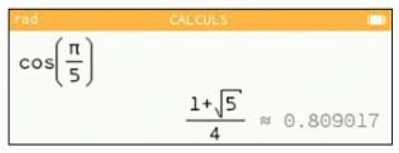
\includegraphics[scale=0.8]{1.02.05-Img01}

En admettant que cette réponse est correcte, en déduire la valeur exacte de chacun des nombres suivants.
\begin{enumMet}
	\item $\cos \left(\dfrac{6 \pi}{5}\right)$
	\begin{corrBox}
		Pour cet exercice, on fait \guillemets{comme si}, on rajoutait 1 valeur dans le tableau des valeurs particulières
		$$
		\cos \left(\dfrac{\pi}{5}\right)=\dfrac{1+\sqrt{5}}{4}
		$$
		
		$\dfrac{6 \pi}{5}=\dfrac{\pi}{5}+\dfrac{5 \pi}{5}=\dfrac{\pi}{5}+\pi$ donc  $\cos \left(\dfrac{6 \pi}{5}\right)=\cos \left(\dfrac{\pi}{5}+\pi\right)=-\cos \left(\dfrac{\pi}{5}\right)=-\dfrac{1+\sqrt{5}}{4}$		
	\end{corrBox}
	\item $\cos \left(-\dfrac{\pi}{5}\right)$
	\begin{corrBox}
		$\cos \left(-\dfrac{\pi}{5}\right)=\cos \left(\dfrac{\pi}{5}\right)$ car $\cos (-x)=\cos (x)$ donc 
		$$
		\cos \left(-\dfrac{\pi}{5}\right)=\dfrac{1+\sqrt{5}}{4}
		$$
	\end{corrBox}
	\item $\sin \left(\dfrac{\pi}{5}\right)$
	\begin{corrBox}
		$\cos ^2\left(\dfrac{\pi}{5}\right)+\sin ^2\left(\dfrac{\pi}{5}\right)=1$
		donc 
		
		$\sin ^2\left(\dfrac{\pi}{5}\right)=1-\cos ^2\left(\dfrac{\pi}{5}\right)=1-\left(\dfrac{1+\sqrt{5}}{4}\right)^2=1-\dfrac{1+2 \sqrt{5}+5}{16}=\dfrac{16}{16}-\dfrac{6+26 \sqrt{5}}{16}=\dfrac{10-2 \sqrt{5}}{16}$
		
		D'ou : $\sin \left(\dfrac{\pi}{5}\right)=\dfrac{\sqrt{10-2 \sqrt{5}}}{4}$
				
	\end{corrBox}
	\item $\sin \left(\dfrac{3 \pi}{10}\right)$
	\begin{corrBox}
		$\begin{array}{r}\dfrac{3 \pi}{10}=-\dfrac{\pi}{5}+\dfrac{\pi}{2}=\dfrac{\pi}{2}-\dfrac{\pi}{5} \text { d'ou } \sin \left(\dfrac{3 \pi}{10}\right)=\cos \left(\dfrac{\pi}{5}\right)=\dfrac{1+\sqrt{5}}{4} \\ \text { car } \cos (x)=\sin \left(\dfrac{\pi}{2}-x\right)\end{array}$		
	\end{corrBox}
\end{enumMet}

\exercice{}

Une saisie calculatrice donne:

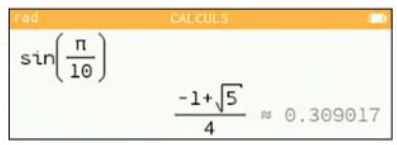
\includegraphics[scale=0.8]{1.02.05-Img02}

En admettant que cette réponse est correcte, en déduire la valeur exacte de chacun des nombres suivants.
\begin{enumMet}
	\item $\sin \left(-\dfrac{\pi}{10}\right)$
	\begin{corrBox}
		$\sin \left(-\dfrac{\pi}{10}\right)=-\sin \left(\dfrac{\pi}{10}\right)=\dfrac{1-\sqrt{5}}{4}$ car $\sin (-x)=-\sin (x)$
		
	\end{corrBox}
	\item $\cos \left(\dfrac{\pi}{10}\right)$
	\begin{corrBox}
		$\cos ^2\left(\dfrac{\pi}{10}\right)+\sin ^2\left(\dfrac{\pi}{10}\right)=1$ d'ou
		
		$\cos ^2\left(\dfrac{\pi}{10}\right)=1-\left(\dfrac{-1+\sqrt{5}}{4}\right)^2=\dfrac{16}{16}-\dfrac{1-2 \sqrt{5}+5}{16}=\dfrac{10-2 \sqrt{5}}{16}$
		
		donc $\cos \left(\dfrac{\pi}{10}\right)=\dfrac{\sqrt{10-2 \sqrt{5}}}{4}$
		
	\end{corrBox}
	\item $\sin \left(\dfrac{2 \pi}{5}\right)$
	\begin{corrBox}
		$\dfrac{2 \pi}{5}=\dfrac{\pi}{2}-\dfrac{\pi}{10}$ d'ou $\sin \left(\dfrac{2 \pi}{5}\right)=\sin \left(\dfrac{\pi}{2}-\dfrac{\pi}{10}\right)=\cos \left(\dfrac{\pi}{10}\right)=\dfrac{\sqrt{10-2 \sqrt{5}}}{4}$ car $\sin \left(\dfrac{\pi}{2}-x\right)=\cos (x)$
		
	\end{corrBox}
	\item $\sin \left(\dfrac{9 \pi}{10}\right)$
	\begin{corrBox}
		$\dfrac{9 \pi}{10}=\pi-\dfrac{\pi}{10}$ donc $\sin \left(\dfrac{9 \pi}{10}\right)=\sin \left(\dfrac{\pi}{10}\right)=\dfrac{-1+\sqrt{5}}{4}$ car $\sin (\pi-x)=\sin (x)$
	\end{corrBox}
\end{enumMet}

\exercice{}

Sans calculatrice, calculer et réduire au même dénominateur les expressions suivantes. On pourra s'aider du cercle trigonométrique et on indiquera les étapes intermédiaires.
\begin{enumMet}
	\item $\cos \left(\dfrac{-\pi}{3}\right)-\sin \left(\dfrac{-7 \pi}{4}\right)$
	\begin{corrBox}
		$\cos \left(\dfrac{-\pi}{3}\right)=\cos \left(\dfrac{\pi}{3}\right) \quad \dfrac{-7 \pi}{4}$ a comme mesure principale $\dfrac{\pi}{4}$ donc $\sin \left(\dfrac{-7 \pi}{4}\right)=\sin \left(\dfrac{-\pi}{4}\right)$
		$$
		\begin{aligned}
			\cos \left(\dfrac{-\pi}{3}\right)-\sin \left(\dfrac{-7 \pi}{4}\right) & =\cos \left(\dfrac{\pi}{3}\right)-\sin \left(\dfrac{\pi}{4}\right) \\
			& =\dfrac{1}{2}-\dfrac{\sqrt{2}}{2}=\dfrac{1-\sqrt{2}}{2}
		\end{aligned}
		$$		
	\end{corrBox}
	\item $\cos \left(\dfrac{5 \pi}{3}\right)-\sin (2 \pi)+\cos \left(\dfrac{-\pi}{6}\right)$
	\begin{corrBox}
		$\dfrac{5 \pi}{3}$ a comme mesure principale $-\dfrac{\pi}{3}$
		$$
		\begin{aligned}
			\cos \left(\dfrac{5 \pi}{3}\right)=\cos \left(\dfrac{-\pi}{3}\right)=\cos \left(\dfrac{\pi}{3}\right) & \sin (2 \pi)=\sin (0)=0 \\
			\cos \left(\dfrac{-\pi}{6}\right)=\cos \left(\dfrac{\pi}{6}\right) & \\
			\cos \left(\dfrac{5 \pi}{3}\right)-\sin (2 \pi)+\cos \left(\dfrac{-\pi}{6}\right) & =\cos \left(\dfrac{\pi}{3}\right)-\sin (0)+\cos \left(\dfrac{\pi}{6}\right) \\
			& =\dfrac{1}{2}-0+\dfrac{\sqrt{3}}{2}=\dfrac{1+\sqrt{3}}{2}
		\end{aligned}
		$$		
	\end{corrBox}
	\item $\cos (-2018 \pi)-\cos \left(\dfrac{-\pi}{4}\right)+\sin \left(\dfrac{3 \pi}{2}\right)-\sin \left(\dfrac{\pi}{4}\right)$
	\begin{corrBox}
		$\cos (-2018 \pi)=\cos (0)$
		$$
		\cos \left(\dfrac{-\pi}{4}\right)=\cos \left(\dfrac{\pi}{4}\right)
		$$
		$\dfrac{3 \pi}{2}$ a comme mesure principale $-\dfrac{\pi}{2}$
		donc $\sin \left(\dfrac{3 \pi}{2}\right)=\sin \left(\dfrac{-\pi}{2}\right)=-\sin \left(\dfrac{\pi}{2}\right)$
		$$
		\cos (-2018 \pi)-\cos \left(\dfrac{-\pi}{4}\right)+\sin \left(\dfrac{3 \pi}{2}\right)-\sin \left(\dfrac{\pi}{4}\right)
		$$
		$=\cos (0)-\cos \left(\dfrac{\pi}{4}\right)-\sin \left(\dfrac{\pi}{2}\right)-\sin \left(\dfrac{\pi}{4}\right)$
		$$
		\begin{aligned}
			& =1-\dfrac{\sqrt{2}}{2}-1-\dfrac{\sqrt{2}}{2} \\
			& =\dfrac{-2 \sqrt{2}}{2}=-\sqrt{2}
		\end{aligned}
		$$
	\end{corrBox}
	\item $\cos \left(\dfrac{\pi}{6}\right)+\sin \left(\dfrac{\pi}{3}\right)-\sin \left(\dfrac{\pi}{2}\right)+\sin \left(\dfrac{4 \pi}{3}\right)$
	\begin{corrBox}
		$\dfrac{4 \pi}{3}$ a comme mesure principale $\dfrac{-2 \pi}{3}$
		$$
		\begin{aligned}
			& -\dfrac{2 \pi}{3}=\dfrac{\pi}{3}-\pi \quad \operatorname{don} c \sin \left(\dfrac{4 \pi}{3}\right)=\sin \left(\dfrac{-2 \pi}{3}\right)=-\sin \left(\dfrac{\pi}{3}\right) \\
			& \cos \left(\dfrac{\pi}{6}\right)+\sin \left(\dfrac{\pi}{3}\right)-\sin \left(\dfrac{\pi}{2}\right)+\sin \left(\dfrac{4 \pi}{3}\right) \\
			& =\cos \left(\dfrac{\pi}{6}\right)+\sin \left(\dfrac{\pi}{3}\right)-\sin \left(\dfrac{\pi}{2}\right)-\sin \left(\dfrac{\pi}{3}\right) \\
			& =\dfrac{\sqrt{3}}{2}+\dfrac{\sqrt{3}}{2}-1-\dfrac{\sqrt{3}}{2}=\dfrac{\sqrt{3}}{2}
		\end{aligned}
		$$				
	\end{corrBox}
\end{enumMet}

\exercice{}

Sans calculatrice, calculer les expressions suivantes. On pourra s'aider du cercle trigonométrique et on indiquera les étapes intermédiaires s'il y en a.
\begin{enumMet}
	\item $\cos ^2\left(\dfrac{-\pi}{13}\right)+\sin ^2\left(\dfrac{-\pi}{13}\right)$
	\begin{corrBox}
		$\cos ^2\left(\dfrac{-\pi}{13}\right)+\sin ^2\left(\dfrac{-\pi}{13}\right)=1$ car $\cos ^2 x+\sin ^2 x=1$	
	\end{corrBox}
	\item $\cos ^2\left(\dfrac{-\pi}{6}\right)-\sin ^2\left(\dfrac{-\pi}{6}\right)$
	\begin{corrBox}
		$\cos ^2\left(\dfrac{-\pi}{6}\right)-\sin ^2\left(\dfrac{-\pi}{6}\right)=\left(\dfrac{\sqrt{3}}{2}\right)^2-\left(\dfrac{1}{2}\right)^2=\dfrac{3-1}{4}=\dfrac{2}{4}=\dfrac{1}{2}$
	\end{corrBox}
	\item $\sin \left(\dfrac{-5 \pi}{6}\right) \times \cos \left(\dfrac{2 \pi}{3}\right)-\cos (-\pi)$
	\begin{corrBox}
		$-\dfrac{5 \pi}{6}=\dfrac{\pi}{6}-\pi$ donc $\sin \left(\dfrac{-5 \pi}{6}\right)=-\sin \left(\dfrac{\pi}{6}\right)$
		et $\cos (-\pi)=\cos (\pi)$
		
		$\dfrac{2 \pi}{3}=\pi-\dfrac{\pi}{3}$ donc $\cos \left(\dfrac{2 \pi}{3}\right)=-\cos \left(\dfrac{\pi}{3}\right)$
		$$
		\begin{aligned}
			\sin \left(\dfrac{-5 \pi}{6}\right) \times \cos \left(\dfrac{2 \pi}{3}\right)-\cos (-\pi) & =-\sin \left(\dfrac{\pi}{6}\right) \times\left(-\cos \dfrac{\pi}{3}\right)-\cos (\pi) \\
			& =\dfrac{1}{2} \times \dfrac{1}{2}-0=\dfrac{1}{4}
		\end{aligned}
		$$					
	\end{corrBox}
	\item $\dfrac{\sin \left(\dfrac{\pi}{4}\right)}{\cos ^2\left(\dfrac{\pi}{3}\right)}$
	\begin{corrBox}
		$\dfrac{\sin \left(\dfrac{\pi}{4}\right)}{\cos ^2\left(\dfrac{\pi}{3}\right)}=\dfrac{\dfrac{\sqrt{2}}{2}}{\left(\dfrac{1}{2}\right)^2}=\dfrac{\dfrac{\sqrt{2}}{2}}{\dfrac{1}{4}}=\dfrac{\sqrt{2}}{2}\times 4=2\sqrt{2}$
	\end{corrBox}
\end{enumMet}


\end{document}

